\documentclass{siproblemset}

\usepackage{multicol}
\usepackage{xcolor}

% SI Session Information
\course{MTH 1321}
\sessionnum{8}
\sessiondate{2/17/22}

\warmup{Concept Review}
\topic{Formal Definition of the Derivative}
\topic{Introduction to Derivative Uses}
\topic{Derivatives of Functions}
\cooldown{Look Back, Look Forward}

% Worksheet Information
\title{Definition of the Derivative, Part 2}
\sections{Section 3.2}
\withnamespace

\begin{document}
    \maketitle
    
    \activity{Warmup}{Concept Overview}{Work with a \textbf{partner} to answer these questions. Try not to use your notes.}{15 minutes}
    
    \frq{What is the limit definitions of the derivative?}
    \smallsp
    
    \frq{What does $f'(x)$ represent both numerically and graphically?}
    \smallsp
    
    \mcq[2]{Evaluate the following derivatives.}{
        \task $\dddx\left[cx\right]=$
        \task $\dddx\left[c\right]=$
        \task $\dddx\left[x^n\right]=$
        \task $\dddx\left[e^x\right]=$
        \task $\dddx\left[f(x)+g(x)\right]=$
        \task $\dddx\left[f(x)-g(x)\right]=$
    }

    \mcq[3]{Determine if the following functions are differentiable at $x=0$. If not, state why.}{
        \task $f(x)=x^2+3$
        \task $g(x)=|x|$
        \task $h(x)=\dfrac1x$
    }
    
    \pagebreak
    \activity{Activity 1}{Limit Definition of the Derivative}{Make a \textbf{group of two or three, all with the same colored worksheets,} to answer your assigned question. Try not to use your notes.}{30 minutes}
    
    \mcq{Determine $f'(x)$ using the limit definition of the derivative.}{
        \task $f(x)=x^2-1$
        \Largesp
        \task $f(x)=\sqrt{x}$
        \Largesp
        \pagebreak
        \task $f(x)=\dfrac{1}{3x-2}$
        \Hugesp 
%        \task $f(x)=x+x^{-1}$
    }
    \pagebreak

    \activity{Activity 2}{Derivative Graphs and Shortcuts}{Make a \textbf{{\em new} group of three, all with the different colored worksheets,} to answer these questions. Try not to use your notes.}{30 minutes}
    
    \frq{For the following graphs, find each function and its derivative.}
    
    \begin{multicols}{2}
        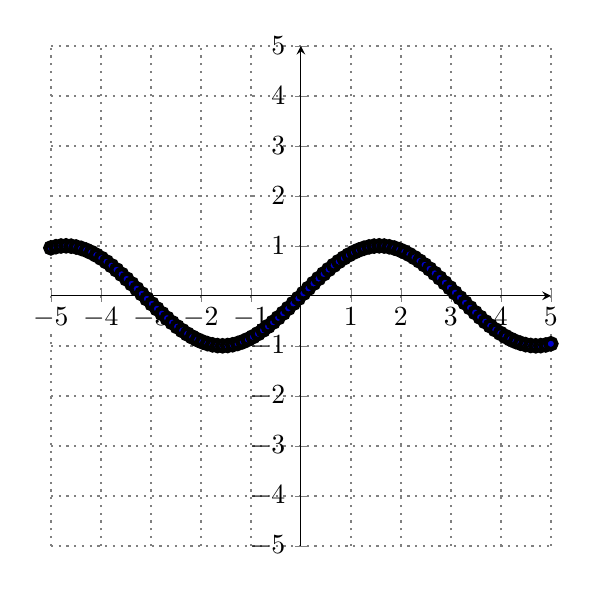
\begin{tikzpicture}
            \begin{axis}[axis x line=center, axis y line=middle,
                width=2.5in, height=2.5in, 
                scale only axis, %axis equal,
                xmin=-5, xmax=5,
                ymin=-5, ymax=5,
                xtick={-5,...,5}, ytick={-5,...,5},
                xticklabel style={draw=none, inner sep=2pt, fill=white, text opacity=1},
                xlabel={}, ylabel={},
                grid=both, grid style={line width=.8pt, draw=gray, dotted},
                minor tick num=0, 
                samples=100]
                \addplot+[black, ultra thick, domain=-5:5] {sin(x*180/pi)};
            \end{axis}
        \end{tikzpicture}
    
        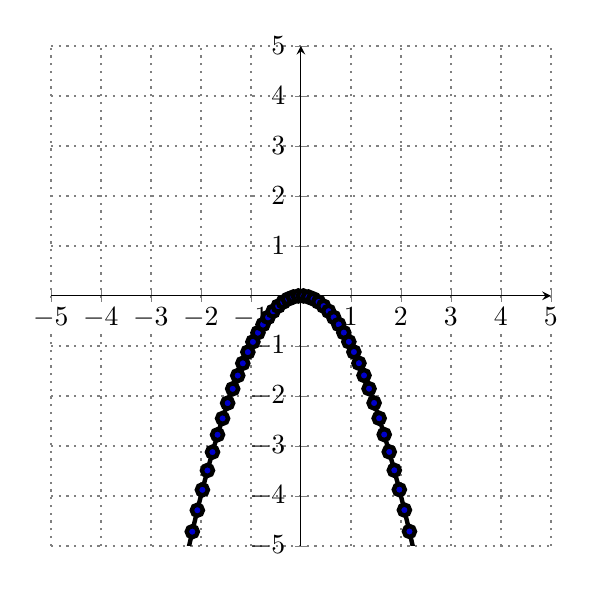
\begin{tikzpicture}
            \begin{axis}[axis x line=center, axis y line=middle,
                width=2.5in, height=2.5in, 
                scale only axis, %axis equal,
                xmin=-5, xmax=5,
                ymin=-5, ymax=5,
                xtick={-5,...,5}, ytick={-5,...,5},
                xticklabel style={draw=none, inner sep=2pt, fill=white, text opacity=1},
                xlabel={}, ylabel={},
                grid=both, grid style={line width=.8pt, draw=gray, dotted},
                minor tick num=0, 
                samples=100]
                \addplot+[black, ultra thick, domain=-5:5] {-x^2};
            \end{axis}
        \end{tikzpicture}
    
        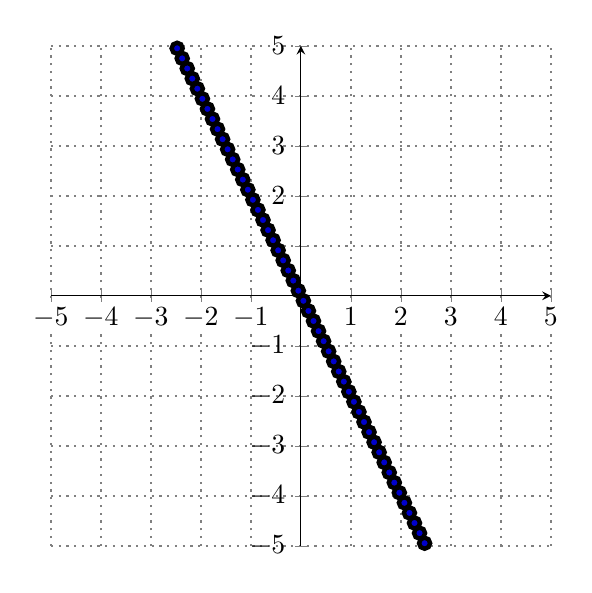
\begin{tikzpicture}
            \begin{axis}[axis x line=center, axis y line=middle,
                width=2.5in, height=2.5in, 
                scale only axis, %axis equal,
                xmin=-5, xmax=5,
                ymin=-5, ymax=5,
                xtick={-5,...,5}, ytick={-5,...,5},
                xticklabel style={draw=none, inner sep=2pt, fill=white, text opacity=1},
                xlabel={}, ylabel={},
                grid=both, grid style={line width=.8pt, draw=gray, dotted},
                minor tick num=0, 
                samples=100]
                \addplot+[black, ultra thick, domain=-5:5] {-2*x};
            \end{axis}
        \end{tikzpicture}
    
        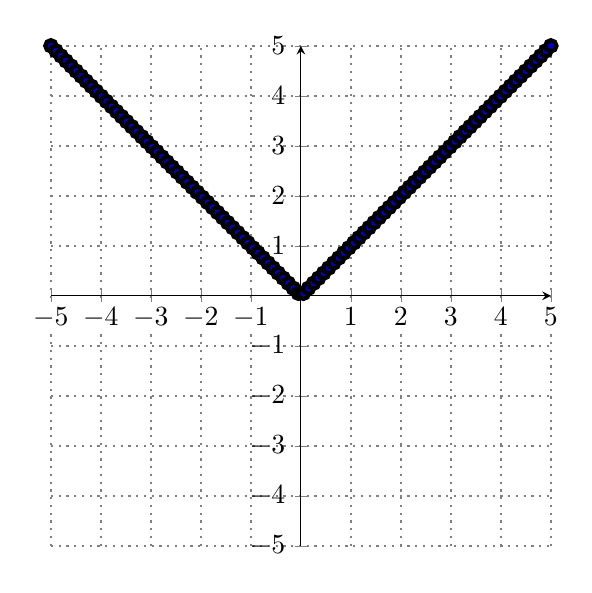
\begin{tikzpicture}
            \begin{axis}[axis x line=center, axis y line=middle,
                width=2.5in, height=2.5in, 
                scale only axis, %axis equal,
                xmin=-5, xmax=5,
                ymin=-5, ymax=5,
                xtick={-5,...,5}, ytick={-5,...,5},
                xticklabel style={draw=none, inner sep=2pt, fill=white, text opacity=1},
                xlabel={}, ylabel={},
                grid=both, grid style={line width=.8pt, draw=gray, dotted},
                minor tick num=0, 
                samples=100]
                \addplot+[black, ultra thick, domain=-5:5] {abs(x)};
            \end{axis}
        \end{tikzpicture}
    
        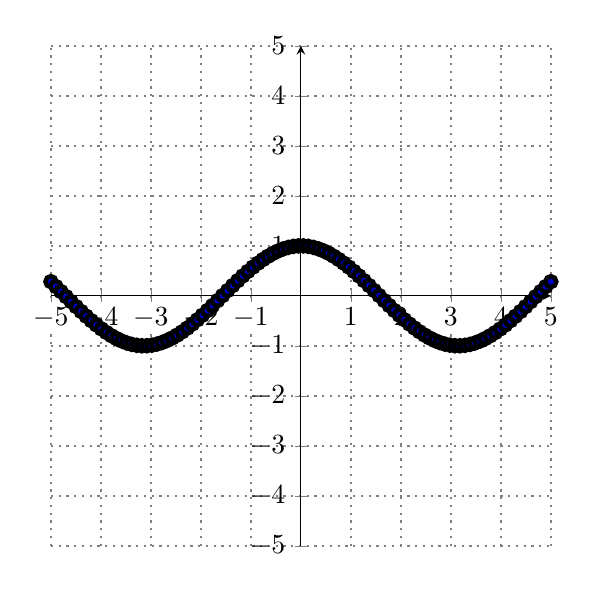
\begin{tikzpicture}
            \begin{axis}[axis x line=center, axis y line=middle,
                width=2.5in, height=2.5in, 
                scale only axis, %axis equal,
                xmin=-5, xmax=5,
                ymin=-5, ymax=5,
                xtick={-5,...,5}, ytick={-5,...,5},
                xticklabel style={draw=none, inner sep=2pt, fill=white, text opacity=1},
                xlabel={}, ylabel={},
                grid=both, grid style={line width=.8pt, draw=gray, dotted},
                minor tick num=0, 
                samples=100]
                \addplot+[black, ultra thick, domain=-5:5] {cos(x*180/pi)};
            \end{axis}
        \end{tikzpicture}
    
        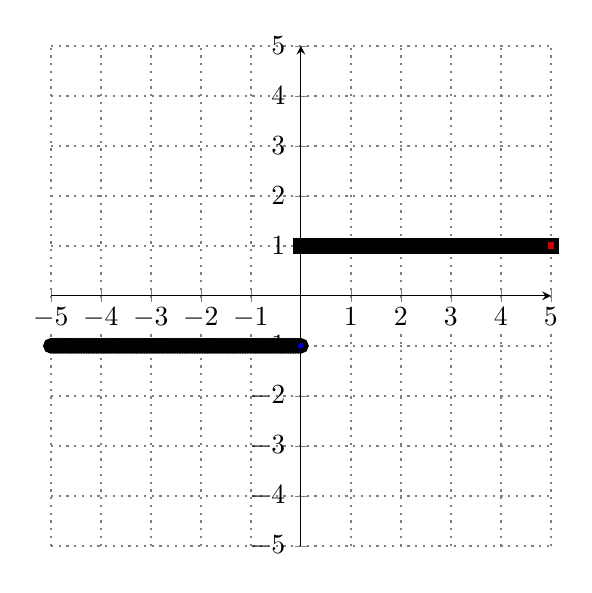
\begin{tikzpicture}
            \begin{axis}[axis x line=center, axis y line=middle,
                width=2.5in, height=2.5in, 
                scale only axis, %axis equal,
                xmin=-5, xmax=5,
                ymin=-5, ymax=5,
                xtick={-5,...,5}, ytick={-5,...,5},
                xticklabel style={draw=none, inner sep=2pt, fill=white, text opacity=1},
                xlabel={}, ylabel={},
                grid=both, grid style={line width=.8pt, draw=gray, dotted},
                minor tick num=0, 
                samples=100]
                \addplot+[black, ultra thick, domain=-5:0] {-1};
                \addplot+[black, ultra thick, domain=0:5] {1};
            \end{axis}
        \end{tikzpicture}
    \end{multicols}
    
    \pagebreak
    
    \mcq{Compute the derivative using any method.}{
        \task $f(x)=x^3$
        \Tinysp
        \task $g(x)=\dfrac{1}{x^4}$
        \Tinysp
        \task $h(x)=x^2-1$
        \Tinysp
        \task $s(t)=7t^3-2t+4$
        \Tinysp
        \task $v(t)=e^t+t^2$
        \Tinysp
        \task $p(x)=e^\pi+\pi^e+x^e+x^\pi$
        \Tinysp
        \task $y=e^{x+2}$
        \Tinysp
    }
    \pagebreak
    
    \activity{Cooldown}{Look Back, Look Forward}{Attempt to do these problems \textbf{alone} then discuss your answers with the people around you.}{15 minutes}

    \frq{Given the limit below, which represents $\dddx[f]$ at $x=x_0$, find $f(x)$ and $x_0$.}
    $$\lim\limits_{h\to 0}\frac{2e^{5+h}-2e^5}{h}$$
    \Normalsp
    
    \frq{Given the limit below, which represents $\dddf[g]{t}$ at $t=t_0$, find $g(t)$ and $t_0$.}
    $$\lim\limits_{t\to t_0}\frac{t^3+3t-{2}^3-3(2)}{t-2}$$
\end{document}